%% LyX 2.3.1-1 created this file.  For more info, see http://www.lyx.org/.
%% Do not edit unless you really know what you are doing.
\documentclass[10pt,letterpaper,conference]{ieeeconf}
\usepackage[latin9]{inputenc}
\setcounter{secnumdepth}{3}
\setcounter{tocdepth}{3}
\usepackage{color}
\usepackage{float}
\usepackage{calc}
\usepackage{units}
\usepackage{textcomp}
\usepackage{amsmath}
\usepackage{graphicx}
\usepackage[unicode=true,
 bookmarks=true,bookmarksnumbered=false,bookmarksopen=false,
 breaklinks=false,pdfborder={0 0 0},pdfborderstyle={},backref=false,colorlinks=true]
 {hyperref}
\hypersetup{pdftitle={Gaussian Process Based Model-less Control with Q-Learning},
 pdfauthor={Jan Hauser and Daniel Pachner and Vladim�r Havlena},
 pdfkeywords={Gaussian process, Q-Learning, Model-less Controll, Machine Learning}}

\makeatletter

%%%%%%%%%%%%%%%%%%%%%%%%%%%%%% LyX specific LaTeX commands.
\pdfpageheight\paperheight
\pdfpagewidth\paperwidth

\newcommand{\lyxmathsym}[1]{\ifmmode\begingroup\def\b@ld{bold}
  \text{\ifx\math@version\b@ld\bfseries\fi#1}\endgroup\else#1\fi}

\floatstyle{ruled}
\newfloat{algorithm}{tbp}{loa}
\providecommand{\algorithmname}{Algorithm}
\floatname{algorithm}{\protect\algorithmname}

%%%%%%%%%%%%%%%%%%%%%%%%%%%%%% User specified LaTeX commands.
%%%%%%%%%%%%%%%%%%%%%%%%%%%%%%%%%%%%%%%%%%%%%%%%%%%%%%%%%%%%%%%%%%%%%%%%%%%%%%%%
%2345678901234567890123456789012345678901234567890123456789012345678901234567890
%        1         2         3         4         5         6         7         8

% Comment this line out if you need a4paper

%\documentclass[a4paper, 10pt, conference]{ieeeconf}      % Use this line for a4 paper

\IEEEoverridecommandlockouts                              % This command is only needed if 
                                                          % you want to use the \thanks command

\overrideIEEEmargins                                      % Needed to meet printer requirements.

%In case you encounter the following error:
%Error 1010 The PDF file may be corrupt (unable to open PDF file) OR
%Error 1000 An error occurred while parsing a contents stream. Unable to analyze the PDF file.
%This is a known problem with pdfLaTeX conversion filter. The file cannot be opened with acrobat reader
%Please use one of the alternatives below to circumvent this error by uncommenting one or the other
%\pdfobjcompresslevel=0
%\pdfminorversion=4

% See the \addtolength command later in the file to balance the column lengths
% on the last page of the document

% The following packages can be found on http:\\www.ctan.org
%\usepackage{graphics} % for pdf, bitmapped graphics files
%\usepackage{epsfig} % for postscript graphics files
%\usepackage{mathptmx} % assumes new font selection scheme installed
%\usepackage{times} % assumes new font selection scheme installed
%\usepackage{amsmath} % assumes amsmath package installed
\usepackage{amssymb}  % assumes amsmath package installed

\title{\LARGE \bf
 Gaussian Process Based Model-less Control with Q-Learning*
}


\author{Jan Hauser$^{1}$ and Daniel Pachner$^{2}$ and Vladim�r Havlena$^{1}$% <-this % stops a space
\thanks{*This work was supported by ...?}% <-this % stops a space
\thanks{$^{1}$Jan Hauser and Vladim�r Havlena are with Department of Control Engineering, 
Faculty of Electrical Engineering of Czech Technical University in Prague, Technicka 2, 166 27 Praha 6, Czech Republic.
Email: {\tt\small \{hauseja3,havlena\}@fel.cvut.cz}}%
\thanks{$^{2}$Daniel Pachner is with Honeywell ACS Global Laboratory Prague, 
V Parku 2326/18, 148 00 Prague, Czech Republic 
Email: {\tt\small daniel.pachner@honeywell.com}}%
}

\makeatother

\begin{document}
\maketitle \thispagestyle{empty} \pagestyle{empty}
\begin{abstract}
The aim of this paper is to demonstrate how Machine Learning (ML)
based on Gaussian Process Regression (GPR) can be used as a practical
control design technique. An optimized control law for a nonlinear
process is found directly by training the algorithm on noisy data
collected from the process when controlled by a sub-optimal controller.
Furthermore, sparse form of GPR is suggested and applied to reduce
computational effort. Simplified nonlinear Fan Coil Unit (FCU) model
is used as an example for which the fan speed control is designed
using the off-policy Q-Learning algorithm. Additionally, the algorithm
properties are discussed, i.e. effect of the sparse GPR, learning
process robustness, GP kernel functions choice. The simulation results
are compared to a simple PI designed based on a linearized model.
\end{abstract}

\section{INTRODUCTION}

Model-less control techniques assume that no mathematical model of
the controlled process is available and the controller is designed
from the measurement data. One such approach would collect the data
in advance during some time window to use it offline for a controller
design. A different approach would attempt to use the data in the
real time to improve the control continuously. In this article the
former offline approach is considered, i.e. the situation when some
sub-optimal controller was already in use and the data were collected
and can be used to optimize, or improve, that controller. Many existing
control design techniques first create a model from data to use it
for a control design method afterwards, which makes sense if some
modeling information, e.g. model structure, is available. A different
approach, used in this paper, is the controller designed directly
from the data, without any process model. This approach can have some
advantages especially if little or nothing is known about the process
or if the process is nonlinear and no simple analytical control design
method is available.

The Q-Learning is an off-policy machine learning (ML) iterative algorithm
\cite{ecc19ref:Sutton_Reinforcement_Learning}, which approximates
certain function satisfying the Bellman equation. This Q function
then defines a controller. To solve problems in continuous state spaces,
Q function can be represented by a universal function approximating
method such as Neural Network or Gaussian Process Regression (GPR).
This approach is very closely related to Markov Decision Process (MDP)
and Approximate Dynamic Programming (ADP) approaches. 

GPR is a non-parametric regression technique \cite{ecc19ref:Rasmussen_Gaussian_Processes}
which is able to approximate any function using noisy data. It can
be applied even if the analytical form of the function is unknown.
Unfortunately, the runtime computational requirement is $\mathcal{O}(n^{3})$
and the memory requirement is $\mathcal{O}(n^{2})$ for $n$ data
points. Various sparse GPR \cite{ecc19ref:Bijl_Online_Sparse_Gaussian},\cite{ecc19ref:Candela_A_unifying_view},{[}\textit{cite:
Guber?}{]} techniques were developed to overcome this computational
complexity. One of the conventional GPR sparse method is to use a
set of size $m$ induction input points which reduces the computational
complexity to $\mathcal{O}(nm^{2})$ (runtime) and $\mathcal{O}(nm)$
(memory). These induction points reduce the whole dataset into a smaller
number of representing data points which are distributed across the
data space to preserve as much information as possible. GP uses various
covariance (kernel) functions \cite{ecc19ref:Williams_Prediction_with_Gaussian_processes}
to define the data covariance matrices. The choice of the kernel can
have significant impact on the accuracy of the regression result.

The contribution of this paper is the practical combination of Q-Learning
and GPR resulting in unbiased estimate of Q function and control policy
improvement. ML algorithms normally needs a large historical dataset
(of size $\sim10^{5}$ and more) to find sufficient result, here a
way smaller dataset is necessary (of a size $\sim10^{3}$). A simple
Fan Coil Unit (FCU) model approximation is used to demonstrate the
approach. FCU is a nonlinear system widely used for both air heating
and cooling in buildings. A linear control design cannot achieve optimal
control in terms of energy consumption and user comfort \cite{ecc19ref:Arguello_Serrano_Nonlinear_HVAC}.
FCU model used here is highly simplified to make the result easier
to interpret.

For reader's understanding, some essential theory is briefly introduced.
In Section \ref{sec:gp}, the GPR algorithm is explained. Moreover,
its sparse approximation is suggested later in text. Section \ref{sec:Q-Learning}
describes the Q-Learning mechanism and how it connects to GPR. In
Section \ref{sec:Fan-Coil-Unit}, a reduced FCU model is explained.
Next Section \ref{sec:RESULTS} presents the results of these techniques
and Section \ref{sec:CONCLUSIONS} concludes and proposes a future
work. 

\section{GAUSSIAN PROCESS\label{sec:gp}}

In this section, GPR method is briefly described. The GPR technique
is then used with Q-Learning algorithm in next section.

\subsection{Gaussian Process Regression}

GPR is a supervised learning regression model, which can be also described
as a distribution over functions \cite{ecc19ref:Rasmussen_Gaussian_Processes}.
It is the function value estimator for an unknown function $f(\mathbf{x})$
considering any dataset $(\mathbf{x},\mathbf{y})$, which can be written
as 

\[
f(\mathbf{x})\sim\mathcal{GP}\left(m(\mathbf{x}),k(\mathbf{x},\mathbf{x}')\right),
\]

\noindent where mean $m(\mathbf{x})$ and covariance function $k(\mathbf{x},\mathbf{x}'$)
are given a priori up to some hyperparameters and are defined as

\begin{eqnarray*}
m(\mathbf{x)} & = & \mathbb{E}\left[f(\mathbf{x})\right],\\
k(\mathbf{x},\mathbf{x'}) & = & \mathbb{E}\left[\left(f(\mathbf{x})-m(\mathbf{x})\right)\left(f(\mathbf{x}')-m(\mathbf{x}')\right)\right],
\end{eqnarray*}

\noindent where $\mathbf{x}$ is a vector representing the dataset
$\mathbf{X}=\left[\mathbf{x}_{1},\mathbf{x}_{2},\ldots,\mathbf{x}_{n}\right]$.

Assume the finite training set $\mathbf{X}$ and the finite testing
set $\mathbf{X}_{*}$, then GPR can predict $f(\mathbf{x}_{j*})$,
where $\mathbf{x}_{j*}\in\mathbf{X}_{*}$, by using data $\mathbf{x}_{i}\in\mathbf{X}$
and their function values $f(\mathbf{x}_{i})$. The function values
$f(\mathbf{X})$ themselves do not need to be accessible but rather
their noisy measurements $\mathbf{y}_{i}=f(\mathbf{X})+\boldsymbol{\varepsilon}_{i}$,
where $\boldsymbol{\varepsilon}$ is a vector of independent identically
distributed (i.i.d) Gaussian noise with variance $\sigma_{n}^{2}$.
The prior covariance of the noisy values is defined as 

\[
\mathrm{cov}(\mathbf{y})=k(\mathbf{X},\mathbf{X})+\sigma_{n}^{2}\mathbf{I}.
\]

Then the prior joint probability distribution function (p.d.f) can
be defined for training and testing sets values as 

\begin{multline*}
\left[\begin{array}{c}
\mathbf{y}\\
f(\mathbf{X}_{*})
\end{array}\right]\sim\\
\mathcal{N}\left(\left[\begin{array}{c}
m(\mathbf{X})\\
m(\mathbf{X}_{*})
\end{array}\right],\left[\begin{array}{cc}
k(\mathbf{X},\mathbf{X})+\sigma_{n}^{2}\mathbf{I} & k(\mathbf{X},\mathbf{X}_{*})\\
k(\mathbf{X}_{*},\mathbf{X}) & k(\mathbf{X}_{*},\mathbf{X}_{*})
\end{array}\right]\right)=\\
\mathcal{N}\left(\left[\begin{array}{c}
\mathbf{m}\\
\mathbf{m}_{*}
\end{array}\right],\left[\begin{array}{cc}
\mathbf{K}_{ff}+\sigma_{n}^{2}\mathbf{I} & \mathbf{K}_{f*}\\
\mathbf{K}_{*f} & \mathbf{K}_{**}
\end{array}\right]\right),
\end{multline*}

\noindent where $\mathbf{K}_{f*}$ is a $n\times n_{*}$ matrix of
the covariances of all pairs of training and testing datasets, i.e.
$\mathbf{K}_{ff}$, $\mathbf{K}_{**}$, $\mathbf{K}_{*f}$ analogously.
Let's also use a notation $\mathbf{\overline{K}}_{aa}=\mathbf{K}_{aa}+\sigma_{n}^{2}\mathbf{I}$
for any $a$. There are many useful covariance functions $k(\mathbf{x},\mathbf{x}')$
called kernels, e.g. squared exponential (SE)

\[
k(\mathbf{x},\mathbf{x}')=\sigma_{f}^{2}\exp\left(-\frac{1}{2l^{2}}\left|\mathbf{x}-\mathbf{x}'\right|^{2}\right)+\sigma_{n}^{2}\delta(\mathbf{x},\mathbf{x}'),
\]

\noindent or polynomial kernel of $d$-degree

\[
k(\mathbf{x},\mathbf{x}')=\left(\mathbf{x}^{\top}\mathbf{x}'+c\right)^{d},
\]

\noindent where $c\geq0$. These kernel functions are also scalable
by their hyperparameters, i.e. these are signal variance $\sigma_{f}^{2}$,
length-scale $l^{2}$ and noise variance $\sigma_{n}^{2}$ for SE
kernel or degree $d$ and soft-margin $c$ for polynomial kernel.

If $\mathbf{y}$ is known, then the posterior conditional normal distribution
of $\mathbf{f_{*}}$ (shortened expression of $f(\mathbf{X}_{*})$)
can be defined. The predictive GPR relationships are following

\begin{eqnarray}
p(\mathbf{f}_{*}|\mathbf{y}) & = & \mathcal{N}(\boldsymbol{\mu}_{*},\mathbf{\Sigma}_{*}),\label{eq:gp-posterior}\\
\boldsymbol{\mu}_{*} & = & \mathbb{E}\left[\mathbf{f_{*}}|\mathbf{y}\right]=\mathbf{m}_{*}+\mathbf{K}_{*f}\overline{\mathbf{K}}_{ff}^{-1}(\mathbf{y}-\mathbf{m}),\label{eq:gp-posterior-mean}\\
\mathbf{\Sigma}_{*} & = & \mathbf{K}_{**}-\mathbf{K}_{*f}\overline{\mathbf{K}}_{ff}^{-1}\mathbf{K}_{f*}.\label{eq:gp-posterior-cov}
\end{eqnarray}

There is an important relationship between the Kalman filter equations
and (\ref{eq:gp-posterior-mean}, \ref{eq:gp-posterior-cov}), this
relationship will be used later. Specifically, we remind that the
term $\mathbf{G}=\mathbf{K}_{*f}\overline{\mathbf{K}}_{ff}^{-1}$
is the Kalman gain matrix. Assuming the unknown function $f$ is a
GP, then training points from dataset $\mathbf{X}$ and the observed
function values $\mathbf{y}$ define the posterior expectations (predictions)
$\mathbf{f}_{*}$ for any test points over a dataset $\mathbf{X}_{*}$.
Unfortunately, these simple calculations can get very expensive due
to the inverse of matrix \textbf{$\overline{\mathbf{K}}_{ff}$}, which
is of size $n\times n$ where $n$ is the number of training data
points. This is the operation which costs $\mathcal{O}(n^{3})$. This
is the moment when sparse GPR is taken into account \cite{ecc19ref:Bijl_Online_Sparse_Gaussian}.

\section{Q-LEARNING\label{sec:Q-Learning}}

This section describes the basic principles of Q-Learning algorithm
\cite{ecc19ref:Sutton_Reinforcement_Learning} which is a model-less
reinforcement learning approach. Then the policy iteration algorithm
based on Bellman equation is introduced. 

For purpose of this section, let's highlight the analogies and slight
differences between two closely related fields: Control Theory (CT),
and MDP respectively. The states $x_{k}$ and inputs $u_{k}$ are
usually considered in CT for a process model, whereas MDP uses the
Markov process states $s_{k}\in\mathbf{S}$ and the agent's actions
$a_{k}\in\mathbf{A}$. Note that the sets $\mathbf{S}$ and $\mathbf{A}$
are usually some real vector spaces in control problems whereas they
may often be finite sets in MDP. The process model itself is an analogy
of probability transition matrix $p(s_{k+1}|a_{k},s_{k})$ of MDP.
Control law, or the state feedback $u_{k}=C(x_{k})$ in CT is an analogy
of a deterministic policy $u_{k}=\pi(s_{k})$. A stochastic policy
defines the joint p.d.f. $\pi(a_{k},s_{k})$ instead of an explicit
function. An important difference exists between the reward $r_{k}(a_{k},s_{k},s_{k+1})$
used in MDP (bounded, to be maximized) and loss function $\ell_{k}(x_{k},u_{k})$
used in CT (often not bounded, to be minimized, almost never depending
on $x_{k+1}$). The ML theory will be discussed below with CT notation.

\subsection{Q Function}

Generally, Q function is a scalar function of a state-input (state-action)
pair which maps to real values 

\[
Q:\mathbf{\mathbf{u\times}x}\rightarrow\mathbb{R}.
\]

It is possible to talk either about Q function $Q^{\pi}(u_{k},x_{k})$
pertaining to a given policy $\pi$ or the Q function $Q^{*}(x_{k},u_{k})$
achieved after convergence. $Q$ (and $Q^{*}$) describes the expected
total discounted loss $\ell(u_{k,}x_{k})$ received by the controller
starting from $x_{k}$ with a control action $u_{k}$ and following
with the policy $\pi$ (and optimal $\pi^{*}$) thereafter. $Q^{*}$,
as function of $u_{k}$, is thus a measure of quality of selecting
the control action $u_{k}$ in a given state $x_{k}$. $Q^{*}$ is
minimized by the optimal control action(s) because, it can only be
made worse. There is also an important parallel between $Q$ function
and the value (cost-to-go) function $V$ used in DP. It is also related
to Lyapunov function and stability theory. $V$ is not used for purpose
of this paper. For a policy $\pi$, not necessarily optimal, the Q
is defined

\begin{multline}
Q^{\pi}(u_{k},x_{k})=\\
l(u_{k},x_{k})+\mathbb{E}\left[\left.\sum_{i=1}^{\infty}\gamma^{i}\ell(u_{k+i}^{\pi},x_{k+i})\right|u_{k},x_{k}\right],\label{eq:q-split-sum}
\end{multline}

\noindent where $\gamma\in\left(0,1\right]$ is a discount factor.
Q function $Q^{*}$ is defined as follows

\begin{multline}
Q^{*}(u_{k},x_{k})=\\
l(u_{k},x_{k})+\mathbb{E}\left[\left.\min_{u_{k+i}}\sum_{i=1}^{\infty}\gamma^{i}\ell(u_{k+i},x_{k+i})\right|u_{k},x_{k}\right].\label{eq:q-function-star}
\end{multline}

The relationship between the Q function $Q^{*}$ and the optimal policy
$\pi^{*}$ is

\begin{equation}
\pi^{*}(x_{k})=\arg\min_{u_{k}}Q^{*}(u_{k},x_{k}).\label{eq:q-function-policy}
\end{equation}

The Bellman optimality principle equation (more usually expressed
in terms of $V$) provides the recursive approach for finding the
Q function $Q^{*}$. It follows directly from (\ref{eq:q-split-sum},
\ref{eq:q-function-star}). For some policy $\pi$, function $Q^{\pi}(x_{k},u_{k})$
must satisfy

\begin{multline}
Q^{\pi}(u_{k},x_{k})=\\
\ell(u_{k},x_{k})+\gamma\mathbb{E}\left[\left.Q^{\pi}(u_{k+1}^{\pi},x_{k+1})\right|u_{k},x_{k}\right],\label{eq:q-value-iteration}
\end{multline}

and for optimal policy $\pi^{*}$ analogously by using (\ref{eq:q-function-star}).

\subsection{Policy Iteration\label{subsec:Policy-Iteration}}

Policy iteration algorithm calculates Q function from Bellman equation
for a current policy and then improves the current policy by seeking
for minimum values of $Q_{k}^{\pi}$ with respect to $u_{k}$ for
each $x_{k}$. Such minimizing $u_{k}$ defines the new policy. This
process is repeated until convergence. It converges to the $Q^{*}$
and provides expected cumulative loss, which is finite for the initial
$\pi$. It means the starting policy can be selected randomly but
must be stabilizing in order to ensure the initial $Q^{\pi}$ is finite. 

\subsection{Q-Learning with Gaussian Process Regression}

Last step in this section is to introduce Q-Learning algorithm with
GPR. For finite (in number of states and actions) MDP, the Q-Learning
algorithms approximate the Q function using the observed samples $x_{k},u_{k}$,
which were encountered during interaction with a system. Nice example
of commonly used Q-Learning is state action reward state action or
SARSA \cite{ecc19ref:Sutton_Reinforcement_Learning}.

This paper considers GPR as Q function approximation and then optimize
the control action using (\ref{subsec:Policy-Iteration}). Method
based on GPR is proposed to calculate Q, because the action-state
space is a vector space where f.e. SARSA cannot be used directly.
Let us define the set of training and prediction points for the GPR
as concatenations of points in the action-state space

\begin{gather}
\mathbf{X}_{*}=\left[\begin{array}{c}
u_{1}^{\pi},x_{1}\\
\vdots\\
u_{k}^{\pi},x_{k}^{\pi}
\end{array}\right],\;\mathbf{X}=\left[\begin{array}{c}
u_{0},x_{0}\\
\vdots\\
u_{k-1},x_{k-1}
\end{array}\right].
\end{gather}

Also, the concatenation of the losses will be used

\begin{equation}
\mathbf{\ell}=\left[\begin{array}{c}
\ell_{0}\\
\vdots\\
\ell_{k-1}
\end{array}\right],
\end{equation}

\noindent and let the Q function be a GP with known kernel. The notation
$\mathbf{f}$ for the unknown function used in GPR context will be
preserved

\begin{equation}
\mathbf{f}_{*}=Q^{\pi}(\mathbf{X}_{*}),\quad\mathbf{f}=Q^{\pi}(\mathbf{X}).
\end{equation}

The noisy realization of $\mathbf{f}=\mathbb{\ell+\gamma E}[Q^{\pi}(\mathbf{X}_{*})]$
is $\mathbf{y}=\mathbf{\ell}+\gamma\mathbf{f}_{*}$. Then based on
(\ref{eq:gp-posterior-mean}) and (\ref{eq:q-value-iteration}), the
conditional means are

\begin{multline}
\mathbb{E\left[\mathit{\left.\begin{array}{c}
\mathbf{f}\\
\mathbf{f}_{*}
\end{array}\right|\mathbf{\mathit{\mathbf{y}}}}\right]}=\\
\left[\begin{array}{c}
\mathbf{m}\\
\mathbf{m}_{*}
\end{array}\right]+\left[\begin{array}{c}
\mathbf{K}_{ff}\\
\mathbf{K}_{*f}
\end{array}\right]\overline{\mathbf{K}}_{ff}^{-1}\left(\mathbf{\ell}+\gamma\mathbf{f}_{*}-\mathbf{m}\right).\label{eq:Q-data-update}
\end{multline}

The expression (\ref{eq:Q-data-update}) may seem useless because
the Q estimates depend on $\mathbf{f}_{*}$ true value which we do
not know. Recall that Q function is neither measured nor observed.
However, consider the left hand side equals the true values \textbf{$\mathbf{f}$}
and $\mathbf{f}_{*}$ for $k\rightarrow\infty$ and sufficient excitation
in the action-state space, and when $\mathbf{m}=\mathbf{f}$ and $\mathbf{m}_{*}=\mathbf{f}_{*}$.
From this one gets a system of linear equations the true values satisfy.
This system of linear equations may have one or infinitely many solutions.
One may now use the Kalman filter and GPR analogy to understand that
the latter happens when some of the function values are not observalbe
\cite{ecc19ref:Kwakernaak_linear_optimal_control_systems}. Although
they may be observable in theory, the Kalman gain may be so small
that the system would get ill-conditioned. We propose to regularize
this situation shifting the unobservable poles of the filter from
1 to some stable real pole $(1-\xi)>\gamma$, i.e. slightly to the
left. Practically, this means that the unobservable Q function values
will be estimated as zeros. With this regularization, we have the
following estimates

\begin{equation}
\left[\begin{array}{c}
\hat{\mathbf{f}}\\
\hat{\mathbf{f}}_{*}
\end{array}\right]=\left(\left(1-\xi\right)\left[\begin{array}{cc}
\mathbf{G} & -\gamma\mathbf{G}\end{array}\right]-\xi\mathbf{I}\right)^{-1}\mathbf{G}\mathbf{\ell},\label{eq:Q-unbiased-estimate}
\end{equation}

\noindent with the Kalman gain matrix $\mathbf{G}$ defined as 

\[
\mathbf{G}=\left[\begin{array}{c}
\mathbf{K}_{ff}\\
\mathbf{K}_{*f}
\end{array}\right]\overline{\mathbf{K}}_{ff}^{-1}.
\]

Without proofs we state several statistical properties of the estimates
(\ref{eq:Q-unbiased-estimate}). They are unbiased (under GPR assumptions)
except of the small bias towards zero caused by $\xi>0$. However,
they are not efficient unless $\mathbf{y}-\mathbf{f}$ would be independent
and homeoskedastic. Also, it should be noted that the uncertainty
of this estimate cannot be calculated by (\ref{eq:gp-posterior-cov})
but must be estimated in a different way.

Not only $\hat{\mathbf{f}},\hat{\mathbf{f}}_{*}$ estimates should
be considered for optimization purpose. Also some general points $\hat{\mathbf{f}}_{**}$
are used during seeking for minimum of $Q$ function in order to find
$\pi^{*}$. These points are not part of the dataset. 

The final algorithm is described in (\ref{alg:Q-learning-with-GP}).
The first step (\ref{enu:a-GP-estimate-}) is to find GPR estimate
of $Q^{\pi^{(i)}}$ by using (\ref{eq:Q-unbiased-estimate}). Next
step (\ref{enu:b-policy-iteration}) is to apply (\ref{subsec:Policy-Iteration})
to minimize found $Q^{\pi^{(i)}}$ and find new policy $\pi^{(i+1)}$.
The stop condition is either a number of iterations or a difference
between control policies $\pi^{(i)}$ and $\pi^{(i+1)}$.

\begin{algorithm}
\begin{centering}
\fbox{\parbox[c]{3in}{%
\textbf{Require: $\mathbf{X},\mathbf{X_{*}},\pi^{(1)}$}
\begin{enumerate}
\item \textbf{while }stop condition

\begin{enumerate}
\item $\pi^{(i)}\rightarrow Q^{\pi^{(i)}}(\mathbf{X},\mathbf{X}_{*})$ \label{enu:a-GP-estimate-}
\item $\pi^{(i+1)}\leftarrow\arg\min_{\mathbf{u}}Q^{\pi^{(i)}}$ \label{enu:b-policy-iteration}
\item $i=i+1$
\end{enumerate}
\item \textbf{end}
\end{enumerate}
%
}}
\par\end{centering}
\caption{Q-Learning with GPR \label{alg:Q-learning-with-GP}}
\end{algorithm}

\section{FAN COIL UNIT \label{sec:Fan-Coil-Unit}}

This section introduces the simplified FCU model used for testing
the algorithm from previous section. FCU is a common air conditioning
system which is inherently non-linear \cite{ecc19ref:Arguello_Serrano_Nonlinear_HVAC}.
Usually installed in building interiors, it consists of a speed controllable
electrical fan, a copper coil flown with heating and/or cooling liquid
(a heat exchanger), and an air supply. It mixes the recirculated interior
air with primary (outdoor) air. This air mixture is then heated/cooled
according to the air temperature setpoint error by flowing through
the coil. Then such air is supplied into the interior and mixed. The
goal is to achieve the temperature set-point maintaining the interior
$\mathrm{CO_{2}}$ fraction and relative humidity at acceptable limits.
Except of the obvious air heating and cooling effect, the heat supplied
to or removed from the air can also be related to water evaporation
or condensation in the unit. It thus makes a difference whether a
FCU changes temperature of more air by less or vice versa. This control
problem is significantly complex and non-linear. A model based optimal
controller cannot be supplied by the unit manufacturer because the
process model involves model of the interior, including its volume,
thermal capacities, thermal insulation, solar and thermal load, $\mathrm{CO_{2}}$
and humidity loads. That is why model-less control or ML techniques
may come into consideration. If such controllers could periodically
re-optimize their behavior using ML techniques, a significant amounts
of energy could be saved world wide.

\subsection{Model }

Only the room air temperature $T_{z}$ $\left[\unit{\lyxmathsym{\textdegree}C}\right]$
state is taken into consideration for purpose of this paper. Considering
the perfect air mixing in the interior, it is described by the differential
equation 

\[
\dot{T}_{z}(t)=\frac{f(t)}{V}\left(T_{s}(t)-T_{z}(t)\right)+\frac{q_{L}(t)}{c_{p}V\rho},
\]

\noindent where $T_{s}(t)$ $\left[\unit{\lyxmathsym{\textdegree}C}\right]$
is supply air temperature, $q_{L}(t)$ $\left[W\right]$ is net heat
load/loss, $f(t)$ $\left[\unit{m^{3}/\unit{s}}\right]$ is air flow,
$V$ $\left[\unit{m^{3}}\right]$ is volume of the interior, $\rho$
$[\unit{kg/\unit{m^{3}}}]$ is air density and $c_{p}$$\left[\unit{J/\unit[kg]{K}}\right]$
is air spec. thermal capacity. Let us define the volume independent
control action as $u(t)=\tau f(t)/V$, i.e. the relative fraction
of the air replaced per time unit $\tau$ (e.g. one hour). The supply
air temperature $T_{s}(t)$ is a nonlinear function of air flow $u(t)$.
The nonlinearity of $T_{s}(t)$ for purpose of this paper was approximated
by the rational function

\begin{equation}
T_{s}(t)=\frac{u(t)T_{z}(t)+eT_{0}}{u(k)+e},\label{eq:supply-air-temperature}
\end{equation}

\noindent where $e$ is a heat exchanger size factor and $T_{0}\left[\mathrm{\lyxmathsym{\textdegree}C}\right]$
is the maximum supply air temperature. The nonlinearity models how
the maximum supply air temperature asymptotically decrease from $T_{0}$
(considered $\mathrm{40^{o}C}$) to $T_{z}$ when the air flow increases.
For simplicity, we neglected the primary air. The heat losses were
considered as $\tau q_{L_{0}}/c_{p}V\rho=-7\mathrm{\lyxmathsym{\textdegree}C}$,
i.e. the room temperature would drop by this amount per unit time
if the air-conditioning would be stopped. 

\section{RESULTS\label{sec:RESULTS}}

This section presents the results. Model from Section \ref{sec:Fan-Coil-Unit}
was considered in discrete difference equation form using the Euler
method with the sampling rate $\tau/200$. The policy iteration algorithm
was applied in order to find the optimal control policy. Loss function
$l$ was defined as

\begin{equation}
l(x_{k},u_{k})=(T_{k}-T_{sp})^{2}+u_{k}^{4},\label{eq:loss-calculation}
\end{equation}

\noindent where setpoint temperature was $T_{sp}=22\unit{\lyxmathsym{\textdegree}C}$
. GPR used the product of a polynomial kernel (degree two) and SE
kernel as the kernel function. Recall that product of kernels is again
a kernel. This choice is based on the fact known from linear control
theory \cite{ecc19ref:Kwakernaak_linear_optimal_control_systems}:
a linear model with quadratic loss has quadratic Q. Hence, our choice
defines a locally linear control law.

Training dataset consists of $2,000$ points $\sim10$ hours. $T_{z_{k}}$
is the only state $x_{k}$ of the process. See Fig. (\ref{fig:Q-Learning-training-data}).
The data used for learning were generated by simulation. The control
$u_{k}$ was selected as random bounded input. 

\begin{figure}
\centering{}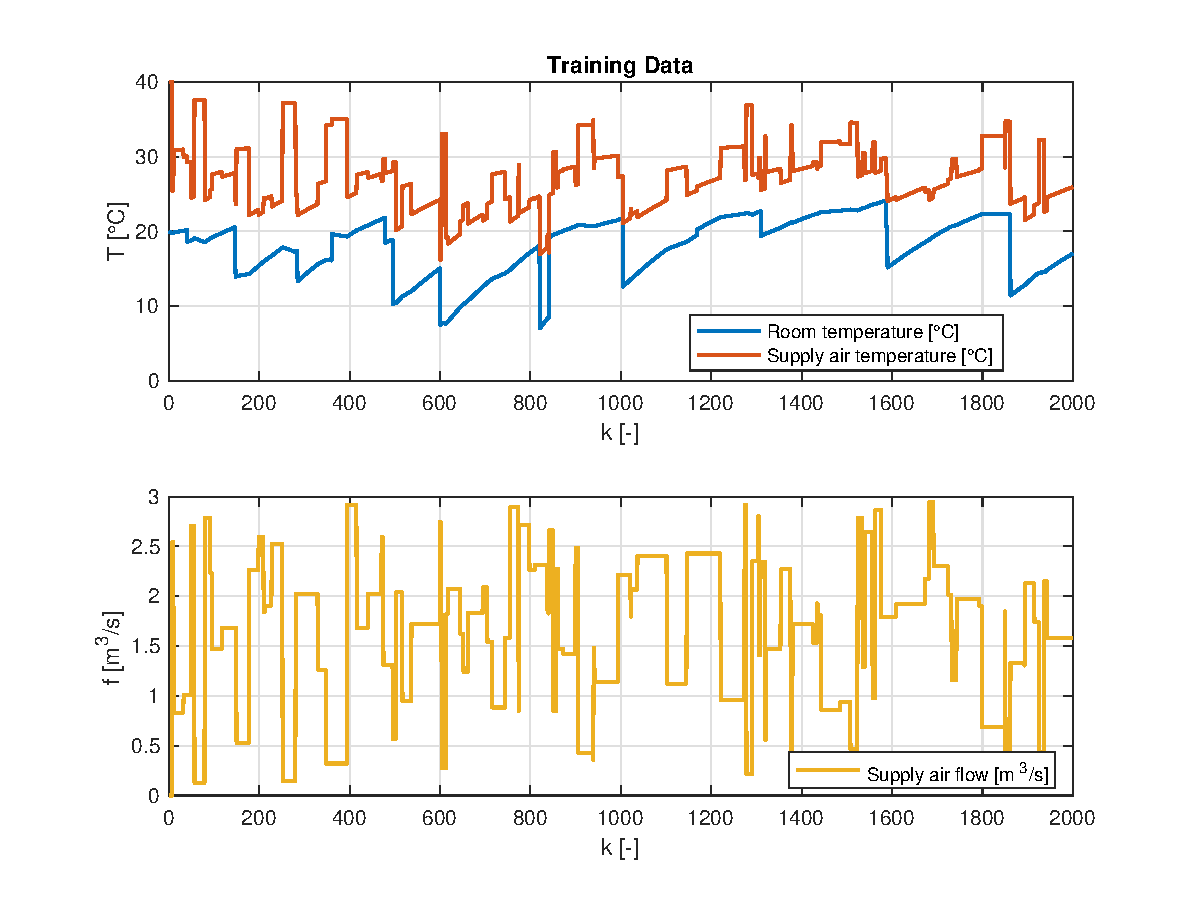
\includegraphics[width=0.95\columnwidth]{figures/training_data}
\caption{\label{fig:Q-Learning-training-data}Q-Learning training data consists
of $2,000$ data points $\sim10$ hours. The room temperature $T_{z_{k}}\sim x_{k}$,
supply air flow rate $u_{k}$, and also supply air temperature $T_{s}$
calculated from (\ref{eq:supply-air-temperature}) shown. }
\end{figure}
Q function was calculated by the proposed method and optimal control
policy $\pi^{*}$ was found after several policy iterations (around
five suffice). Value $\gamma=1-1e^{-3}$ was used in Q-Leatning algorithm.
Also note here, that it is very important to let $u_{k}^{\pi}$ excite
in order to let the algorithm explore more input-state space. This
is well known problem of exploration-exploitation trade-off. Fig.
(\ref{fig:Q-Learning-with-Gaussian}) shows the trajectory of optimal
policy as a curve connecting the minima of Q function with respect
to $u$.

\begin{figure}
\centering{}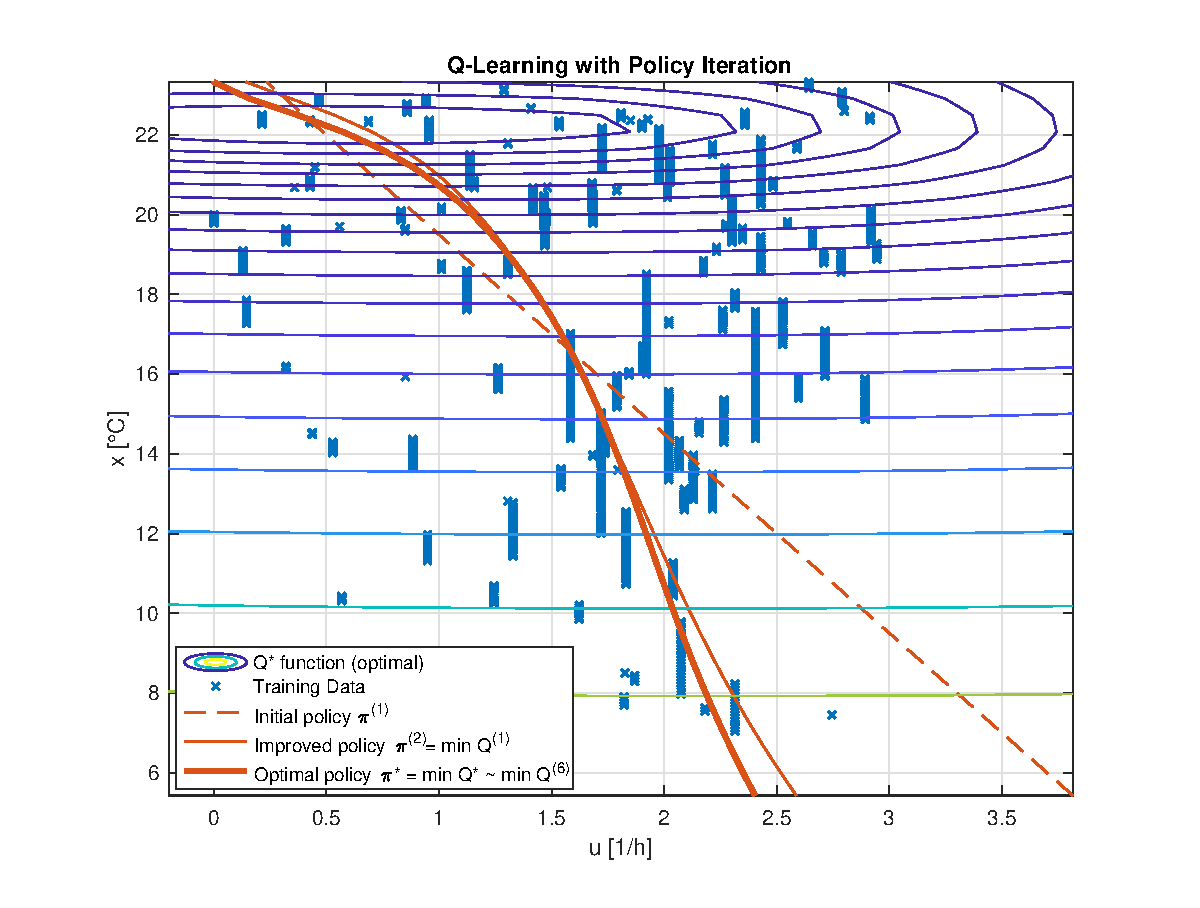
\includegraphics[width=0.95\columnwidth]{figures/q_learning_improved}
\caption{\label{fig:Q-Learning-with-Gaussian}Q-Learning with GPR and Policy
Iteration. Q function $Q^{*}$ is presented and optimal control policy
$\pi^{*}$ was calculated from (\ref{eq:q-function-policy}) and its
curve highlighted here.}
\end{figure}
This Q learning result makes good sense intuitively. The air exchange
rate $u_{k}$ equals the heat losses when the room temperature is
at the set point. Then it increases if the temperature is lower in
order to heat the interior. Therefore, there is a negative feedback
as expected. However, this feedback gain becomes smaller when the
control error is greater because the large air flows are less effective
for heating due to limited heat exchanger effectiveness and the decreasing
supply air temperature. Instead, the electrical fan noise and the
air flow would would just annoy the occupants. Also, the fan would
use more electricity. As such, the policy resembles a proportional
feedback controller with variable gain. It does not have any integral
action whereas a proportional derivative integral (PID) controller
would be normally used for similar purpose. However, it can be shown
that the intergal action can be added to Q learned policy augmenting
the state space with temperature time difference and considering the
time difference $u_{k}-u_{k-1}$ as the control action. Recall that
the integral action is important in order to reject unmeasured slow
disturbances.

\subsection{Q-Learning Evaluation}

The results from Q-Learning were compared to multiple PI controllers
in terms of their cumulative loss function $L$ values. This function
represents the sum of all losses during all episodes, i.e. $L=\sum_{k}\ell_{k}$
and the assuredly optimal value of cumulative loss $L^{*}$ is given
by the optimal policy $\pi^{*}$ from Q learning. A grid of proportional
and integral PI constants was considered so that it obviously contained
the optimal PI values (local minimum). The cumulative loss was calculated
for each in the same way as $L^{*}$ was calculated, i.e. using (\ref{eq:loss-calculation}),
so the cumulative losses are made comparable. The initial room temperature
was $\mathrm{10^{o}C}$ and the cumulative loss was calculated for
1,000 sampling periods. These cumulative loss values were then compared
to $L^{*}$ in Fig. (\ref{fig:Comparison-of-PI-Q-Learning}) and the
best PI controller parameters from the grid were selected for Fig.
(\ref{fig:Q-Learning-PI-PI}). A PI controller designed for a linearized
model of FCU at $u_{0}=1,x_{0}=22\left[\unit{\lyxmathsym{\textdegree}C}\right]$
is also visualized. It can be observed that the best PI almost matches
the result of the Q learning.

\begin{figure}
\centering{}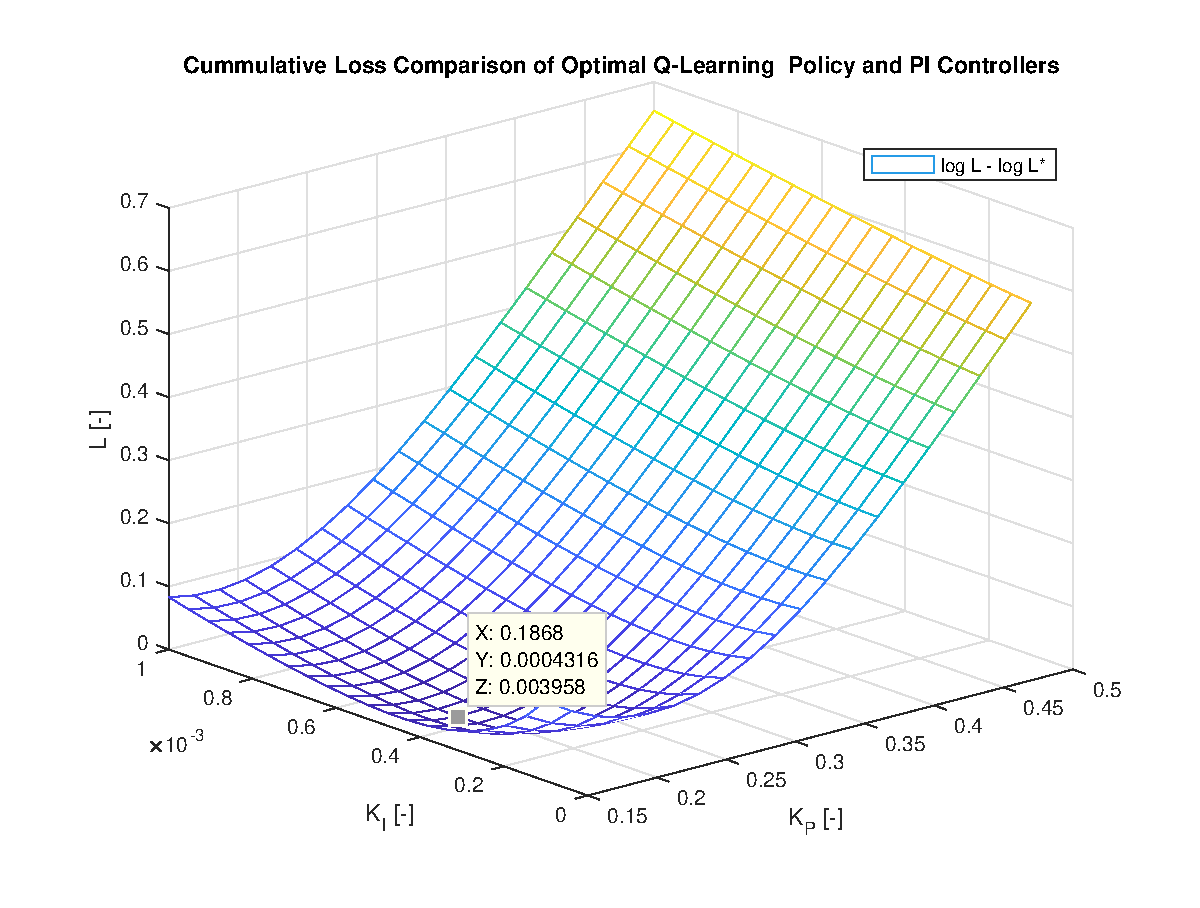
\includegraphics[width=0.95\columnwidth]{figures/q_learning_vs_pi_contr}
\caption{\label{fig:Comparison-of-PI-Q-Learning}Comparison of PI controllers
cumulative losses $L$ with optimal policy cumulative loss $L*$.}
\end{figure}
\begin{figure}
\centering{}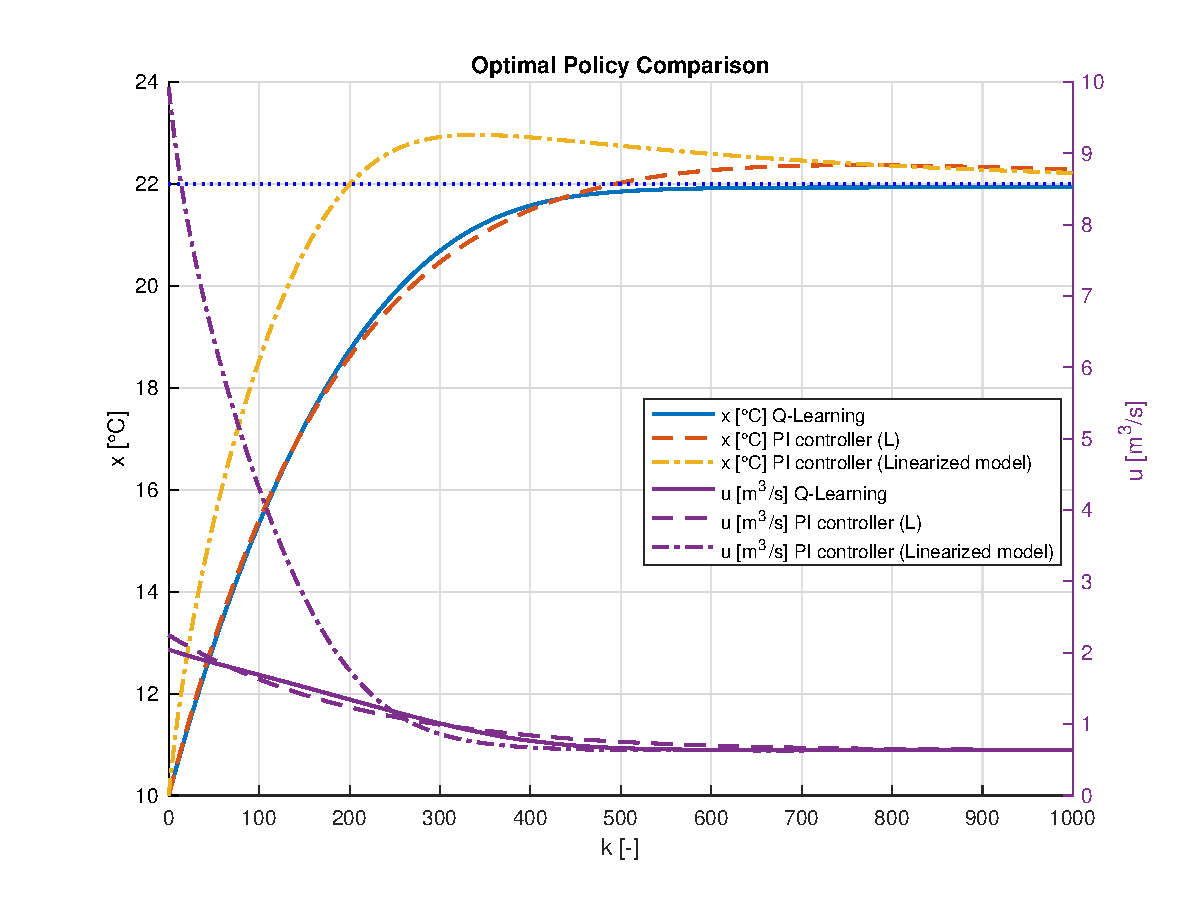
\includegraphics[width=0.95\columnwidth]{figures/optimal_policy}
\caption{\label{fig:Q-Learning-PI-PI}Comparison of Q-Learning optimal control
policy, PI controller designed by cumulative loss comparison and PI
controller designed from linearized model of FCU. The results are
presented on nonlinear FCU model.}
\end{figure}
Next, the controllers and the Q learning were tested considering the
net heat load/heat loss $q_{L}$ not constant but uniformly distributed
over $\left[-7,0\right]$. The result is shown in Fig. (\ref{fig:Q-Learning-PI-PI-noisy}).
Note that Q-Learning designed controller is robust towards such a
noise. It should be noted that the same noise was used to generate
the learning data for this test, not only when simulating the controller.

\begin{figure}
\centering{}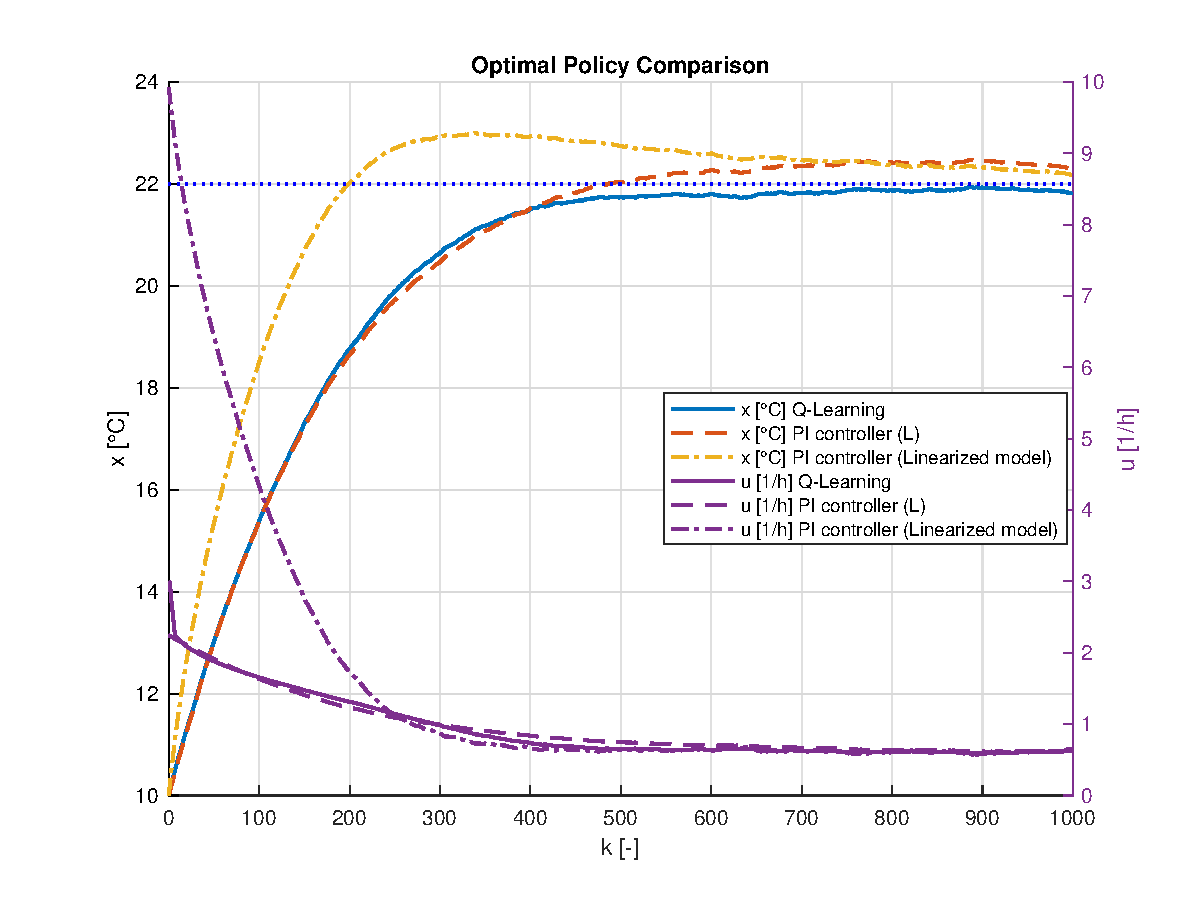
\includegraphics[width=0.95\columnwidth]{figures/optimal_policy_noisy}
\caption{\label{fig:Q-Learning-PI-PI-noisy}Comparison of Q-Learning optimal
control policy, PI controller designed by cumulative loss comparison
and PI controller designed from linearized model of FCU. The results
are presented on nonlinear FCU model with noisy net heat load/heat
loss $q_{L}$.}
\end{figure}
Note, that the dataset size is very important and if only a small
dataset is available, the Q-Learning result degrades significantly. 

\section{CONCLUSIONS\label{sec:CONCLUSIONS}}

This paper described a practical approach of using GPR based Q-Learning
algorithm to find a control law for a completely unknown nonlinear
process based on a historical dataset of size $\sim10^{3}$. Engineers
face such problem often and a solution is of practical interest. GPR
approach was used to estimate Q function value in any point in the
action value space. The policy iterations were used to optimize the
controller as this method converges rapidly. It requires the initial
control to be stabilizing. This does not seem to be a serious constraint
in many practical applications such as building control. The optimal
control law was then fully defined by the minima of Q function $Q^{*}$.
Although not explained in this paper, GPR can be globally minimized
even if the function $f$ is not convex provided the kernel is either
convex after a transformation \cite{ecc19ref:Franey_Branch_and_Bound_Algo}.
It was shown how GPR can be used to get an unbiased Q estimate which
is not sensitive to noise affecting the process. Note that the proposed
method is more accurate than just solving the temporal difference
equation in the least squares sense which results in a bias \cite{ecc19ref:Bratke_Linear_Least_Squares_Algo}.
The approach can be integrated with the GPR sparse form in order to
lower the dimensionality. However, details of this reduction is currently
a subject of research. The approach was tested on a simplified one-input
one-state FCU simulation model and an optimal control policy $\pi^{*}$
was calculated. The result makes sense intuitively, the feedback gain
is gradually decreasing with the control error. A grid of PI controllers
were compared in terms of cumulative loss $L$ with the assuredly
optimal cumulative loss $L^{*}$, which was found by the Q-learning.
The best controller from the grid is slightly worse than $L^{*}$.
Such direct controller optimization may be impractical in reality
because it is very time consuming. Also, another PI controller was
designed based on a linearized FCU model. This traditional approach
could be actually used in practice together with, for example, Ziegler
Nichols PID calibration method. The controllers were compared in Section
\ref{sec:RESULTS} and the performance of both PI found by direct
search and PI designed using linearized FCU were shown to be worse
than Q-Learning policy $\pi^{*}$. The whole process was described
for reader's understanding on the high level. Many technical details
were mentioned just briefly. However, the method is quite simple and
straightforward.

The main pitfalls of the process may be also pointed out. Firstly,
it is necessary to choose several parameters, i. e. the hyperparameters
for GP and the training dataset. Their optimization and diagnostics
is possible and it is current research topic. Although result with
only one kernel (SE times quadratic) was presented, we also tried
different kernels with similar results provided the hyperparameters
were chosen reasonably and the kernels were smooth. Tuning of hyperparameters
is not discussed in this paper. Next interesting problem is the tuning
of sparse GPR parameters. Overall, the method gives reasonably consistent
results not overly sensitive to the data or parameters. 

\bibliographystyle{plain}
\bibliography{ecc19ref}

\end{document}
